\documentclass[a4paper, 12pt]{report}

\title{Editeur web}
\author{Pierre Burc, Olivier Duplouy, Hamza Erraji, Issame Amal, Mickaël Berger, Joachim Divet, Zaydane Sadiki & Abdelhamid Belarbi}

%% Pour des marges plus équitables.
\usepackage[margin=1.5cm]{geometry}
%% Pour la langue des titres et sous-titres.
\usepackage[francais]{babel}
%% Pour de belles images.
\usepackage{graphicx}
%% Pour la police de caractères.
\usepackage{fontspec}
%%\setmainfont{Delicious-Roman}
%% Pour faire le glossaire.
\usepackage{glossaries}
\makeglossaries
%% Après première compilation écrire ligne suivante dans un terminal:
%% miktex-makeindex -s rapportStageAbdel.ist -t rapportStageAbdel.glg -o rapportStageAbdel.gls rapportStageAbdel.glo
%% re-compiler ensuite.
\begin{document}
	%% Glossaire
	\newglossaryentry{UML}
	{
		name=UML,
		description={Unified Modeling Language, langage de modélisation graphique à base de pictogrammes}
	}

	\newglossaryentry{diagramme de Gantt}
	{
		name=diagramme de Gantt,
		description={Le diagramme de Gantt est un outil utilisé en ordonnancement et gestion de projet et permettant de visualiser dans le temps
		les diverses tâches liées composant un projet. Il permet de représenter graphiquement l'avancement du projet}
	}
	
	\newglossaryentry{bogue}
	{
		name=bogue,
		description={En informatique, un bug (de l’anglais bug, « insecte ») ou bogue est un défaut de conception d'un programme
		informatique à l'origine d'un dysfonctionnement},
		plural=bogues
	}
	
	\newglossaryentry{auto-complétion}
	{	
		name=auto-complétion,
		description={L'auto-complétion est une fonctionnalité consistant à compléter automatiquement le mot que l'utilisateur est en train décrire}
	}
	
	\newglossaryentry{workspace}
	{
		name=workspace,
		description={Le workspace est un dossier regroupant l'ensemble des projets créés par l'utilisateur}
	}
	
	\newglossaryentry{coloration syntaxique}
	{
		name=coloration syntaxique
		description={La coloration syntaxique est une fonctionnalité permettant de colorer les mots clés du fichier en cours de lecture en se basant sur son extension}
	}
	
	\begin{titlepage}
		\center{
\includegraphics[width=5cm]{images/logoUM2.png}}	\\ 
		~\\
		~\\
		~\\
		~\\
		~\\		
		\begin{center}
			{\large Rapport de projet} \\
			{\large Licence 3}\\
			\vspace{1,5cm}
			{\Huge Editeur de sites web}\\
			~\\
			~\\
			~\\
			
\includegraphics[width=12.5cm]{images/logoTest1.png}
			~\\
			~\\
			{\large Réalisé par :} \\
			~\\
			{\LARGE Pierre Burc, Olivier Duplouy, \\
				      Hamza Erraji, Issame Amal,\\
				      Mickaël Berger, Joachim Divet,\\
				      Zaydane Sadiki et Abdelhamid Belarbi}\\
			\vspace{1,5cm}
			{\large Sous la direction de:} \\
			~\\
			{\LARGE Michel Meynard} \\
			\vspace{2.5cm}
			{\large Année universitaire 2011-2012 }			
		\end{center}
	\end{titlepage}
%%%%%%%%%%%%%%%%%%%%%%%%%%%%%%%%%%%%%%%%
%%%%%%%%%%%%%%%%%%%%%%%%%%%%%%%%%%%%%%%%
	\begin{chapter}*{Remerciements}
	Nous tenons à remercier tout particulièrement M. Michel Meynard, notre tuteur de projet qui nous a guidés et épaulés tout au long de la réalisation de ce projet. 

	Bien entendu nous n'oublions pas de remercier chaleureusement toute l'équipe pédagogique de l'UM2 qui nous a apporté son soutien.
	\end{chapter} 
%%%%%%%%%%%%%%%%%%%%%%%%%%%%%%%%%%%%%%%%
%%%%%%%%%%%%%%%%%%%%%%%%%%%%%%%%%%%%%%%%
	%% Table des matières.
	\tableofcontents
%%%%%%%%%%%%%%%%%%%%%%%%%%%%%%%%%%%%%%%%
%%%%%%%%%%%%%%%%%%%%%%%%%%%%%%%%%%%%%%%%
	\begin{chapter}*{Introduction}
	\addcontentsline{toc}{chapter}{Introduction}
%% Introduction de Abdelhamid.
	C'est par une froide journée d'hiver que nous nous réunîmes pour la première fois à l'université de Montpellier. 
	Huit, tous étudiants préposés au projet numéro 23 nous attendons à notre table l'arrivée de notre tuteur M. Meynard. 
	Ce dernier se présente, nous salue et prononce ce discours mémorable qui restera gravé à jamais dans les mémoires, du moins cette année.\\
	\begin{quotation}
		``Dans le cadre de développement de sites Web, on souhaiterait utiliser un éditeur multi-fichiers permettant de réaliser différentes actions sur
		des fichiers relatifs à un site: édition de fichiers Html, Php, JavaScript et Css.

		Il serait également appréciable que cet éditeur proposât un mode de visualisation du site dans un navigateur et un mode arborescence.

		On pourrait aussi avoir de l'\gls{auto-complétion}, de la coloration syntaxique, un accès aux manuels des langages cités précédemment et pourquoi
		pas une validation Html.\,''
	\end{quotation}

	Après ce laïus prononcé d'une traite M. Meynard disparut soudain, nous laissant là, le regard vide.\\


	Néanmoins, nous nous remîmes assez vite de notre ahurissement et un sage parmi nous s'écria soudain:
	\begin{quotation}
		``Nous commencerons par étudier quelques éditeurs existants sur le marché pour nous faire une idée. Ensuite nous concevrons
		le programme avec le langage UML en nous organisant pour la réalisation.
		Enfin, nous implémenterons l'application insolents et sûrs de nous.	Qu'en dites-vous ?''
	\end{quotation}

	Nous n'en dîmes que du bien. En effet, l'idée loin d'être incroyablement novatrice avait l'avantage d'être logique et cohérente.

%% Ici commence l'introduction signée Olivier.

	Au début du mois de Février, il nous a été demandé de réaliser un projet ayant pour but de mettre en place une application permettant
	d'utiliser un éditeur multi-fichiers effectuant différentes actions sur des fichiers relatif à un site web.\\
	Ce dernier consiste à créer, modifier, sauvergarder... des fichiers contenant les langages JavaScript, HTML, CSS, PHP via une interface se
	rapprochant des IDEs présents sur le marché. Celle-ci aura un rôle primordial, car elle devra apporter à l'utilisateur une aide précieuse grâce
	à des fonctionnalités intuitives, comme par exemple l'auto-complétion.\\
	A l'occasion de ce projet, un groupe de huit personnes a été formé pour répondre à la capacité de travail demandée. Nous devions donc nous 
	répartir les tâches entre chaque membre voir créer des sous-groupes permettant de cloisonner chaque brique essentielle de l'application 
	(interface,système,coloration/complétion). De plus, une période de trois mois nous a été accordée pour réaliser cet IDE.\\
	Afin de ne pas gaspiller du temps à déterminer par où commencer et de quelle façon aborder le sujet, nous avions des réunions régulières avec 
	notre tuteur M.Meynard, pour nous guider dans notre réflexion.\\
	A travers ce compte-rendu nous essaierons de rendre compte des étapes qui nous ont conduits à élaborer cette application en essayant de répondre 
	le plus fidèlement possible au problème posé.\\ 
	
	\end{chapter}
%%%%%%%%%%%%%%%%%%%%%%%%%%%%%%%%%%%%%%%%
%%%%%%%%%%%%%%%%%%%%%%%%%%%%%%%%%%%%%%%%
	\begin{part}{Analyse}
		\begin{chapter}{Cahier des charges}
		Pour nous donner une idée du rôle que devra jouer notre éditeur web, une liste des principales fonctionnalités nous a été fournie,
		présentée ci-dessous:\\
				\begin{itemize}
					\item Édition des fichiers JavaScript, Php, Css et Html;
					\item Un système multi-onglets permettant de naviguer rapidement entre plusieurs fichiers d'un même projet;
					\item Possibilité de visualiser le site sous forme d'arborescence;
					\item Auto-complétion et coloration syntaxique;
					\item Auto-indentation;
					\item Accès en un clic au manuel Php/Html/Css/JavaScript;
					\item Validation Html;
					\item Visualisation du site dans un navigateur;
					\item Squelette de site préexistant.
				\end{itemize}
		

		 %%C'est pas un peu trop technique par hasard ?		
		Après avoir pris connaissance du cahier des charges initial, nous avons décidé de rajouter quelques spécifications sur certaines 
		fonctionnalités. Concernant la visualisation du site web, 2 possibilités s'offraient à nous. La première était de réserver une fenêtre à 
		l'intérieur de l'application destinée à afficher en temps réel le site web, après chaque modification.
		Nous avons opté pour la seconde solution, qui met à disposition de l'utilisateur un bouton permettant de visualiser le site à 
		travers l'ouverture d'un naviguateur.\\
		Une contrainte a également été ajoutée pour la coloration syntaxique, car nous avons décidé d'obliger l'utilisateur à enregistrer le 
		fichier dés sa création, de manière à récupérer l'extension du fichier pour déterminer le langage utilisé.\\
		
			~\\
		\end{chapter}
		\begin{chapter}{Étude de projets existants}
		\begin{section}{Espresso}
				\begin{figure}[h]
					\begin{center}
						
\includegraphics[width=3cm]{images/logoEspresso.png}
						\caption{Espresso}
					\end{center}
				\end{figure}~\\
				Le premier programme d'édition de site web que nous avons étudié propose les mêmes fonctionnalités que le
				logiciel que nous nous proposons de développer, à savoir coloration syntaxique, indentation automatique, arborescence des codes, etc.
				Il sera à priori une bonne source d'inspiration pour nous d'autant plus que l'interface est très soignée et agréable d'utilisation.
			\end{section}
			~\\
			\begin{section}{Aptana}
				\begin{figure}[h]
					\begin{center}
						
\includegraphics[width=4cm]{images/logoAptana.png}
						\caption{Aptana}
					\end{center}
				\end{figure}~\\
				Cet éditeur propose un ensemble de fonctionnalités nombreuses et variées. Beaucoup plus fourni que Espresso, il propose des fonctionnalités complexes dans divers langages : déboguage, déploiement automatique, gestionnaire de version inclus, terminal intégré et moult autres outils.
				Pour nous c'est un bon modèle à suivre en évitant tout de même de tomber dans le piège du sur-nombre d'options qui importuneraientt l'utilisateur. 
			\end{section}
			~\\
			\begin{section}{Dreamweaver}
				\begin{figure}[h]
					\begin{center}
						
\includegraphics[width=3cm]{images/logoDreamweaver.png}
						\caption{Dreamweaver}
					\end{center}
				\end{figure}~\\
				Dreamweaver est une référence en la matière. Il réunit les atouts des deux éditeurs sus-cités en joignant l'utile à l'agréable.
				Il possède en outre un mode dit WYSIWYG. Derrière ce sigle barbare se cache la possibilité intéressante de dessiner l'interface d'un site web.
				Nous concernant, nous pourrons proposer à l'utilisateur de visualiser le site sur lequel il travaille.
			\end{section}
			~\\
		\end{chapter}
		\begin{chapter}{Choix des outils}
			Avant de nous lancer dans la réalisation de l'application, nous avons du choisir les outils les plus adaptés avec lesquels 
			nous avons conçus et programmer. Dans un premier temps, le langage de programmation devait être absolument choisit. 
			Nous avons pensé au C++ pour plusieurs raisons. D'une part, nous l'avons utilisé durant cette année et est portable, 
			donc un langage maîtrisé par les huit membres du groupe et utilisable sur n'importe quel système d'exploitation sans conflits.
			D'autre part, nous pouvons trouver très facilement beaucoup de documentation à son sujet, et il est également adapté à la 
			réalisation de logiciels. %%%%%%%%%% METTRE IMAGE C++ %%%%%%%%%%
			\\
			Par la suite, nous avons du adopter un IDE permettant de programmer avec le C++. 
			Notre tuteur nous a orienté vers le framework QT Creator, intégrant de multiples bibliothèques utiles pour le projet. 
			De plus, QT offre la possibilité de réaliser des interfaces graphiques grâce à QT Designer, simplifiant grandement la programmation par
			la présence de fonctionnalités déjà toutes faites.%%%%%%%%%% METTRE IMAGE QT %%%%%%%%%%
			\\
			Travaillant en groupe de huit, un gestionnaire de versions était indispensable pour partager les différents travaux effectués
			par chacun des membres. Nous avons donc choisis le gestionnaire de versions GIT, avec une prise en main accessible à tous.
			 %%%%%%%%%% METTRE IMAGE GIT %%%%%%%%%%
			\\
			A côté de la programmation pure, il fallait bien sur pouvoir communiquer entre nous de manière rapide à distance. 
			N'habitant pas tous à Montpellier, il a fallu opter pour une solution collaborative. 
			Le web nous offrant cette possiblité, nous avons sélectionné deux sites:
			\begin{description}
				\item[MicroMobs.com:] Pour les discussions professionnelles;
				\item[Facebook:] Pour les annonces, les dates de réunions,etc...;
			\end{description}~\\
			Enfin, pour la conception et la modélisation des différentes structures à implémenter, nous avons utilisé le site YUML.me
			permettant de concevoir et générer des diagrammes UML. %%%%%%%% METTRE IMAGE YUML %%%%%%%%% 
			De plus, TeamGantt.com nous a été utile pour établir le diagramme de Gantt, et ainsi planifier les différentes 
			étapes du projet et séparer le groupe en plusieurs sous-groupes et savoir approximativement combien de temps nous prendrait chaque tâche.
			\\

		\end{chapter}
		\begin{chapter}{Organisation}
		\begin{section}{Diagramme de Gantt}
			Le projet se déroulant sur quatre mois, il a fallu faire un planning qui s'étale sur ledit laps de temps.
			Voici toutes les étapes du projet inscrites sur un diagramme de Gantt.
				\begin{figure}[h]
					\begin{center}
						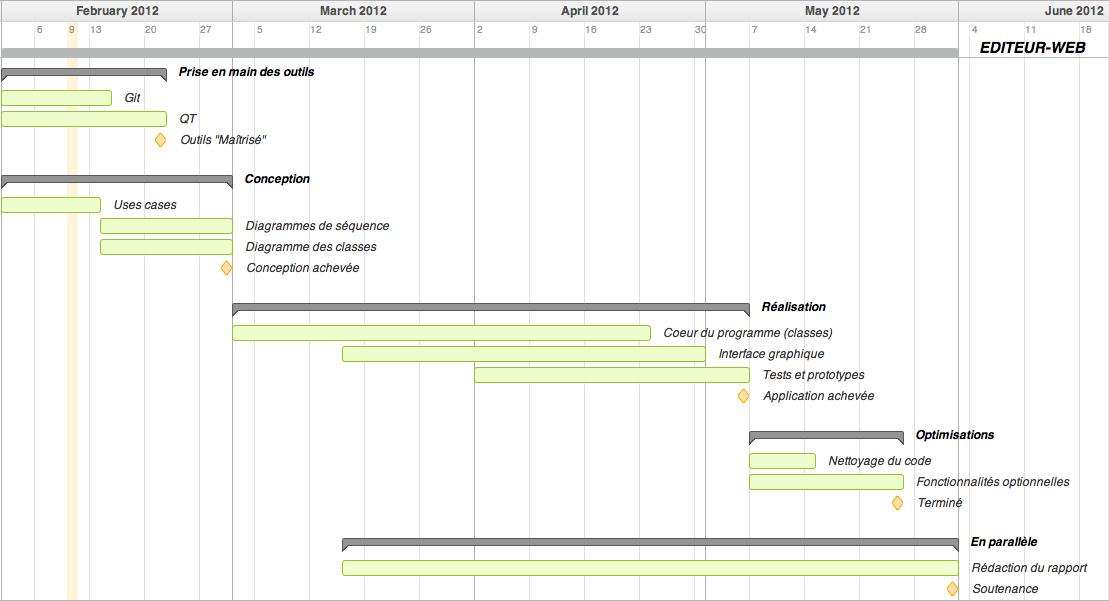
\includegraphics[width=17cm]{DiagrammeGantt.png}
						\caption{Diagramme de Gantt}
					\end{center}
				\end{figure}~\\
			\end{section}
		\end{chapter}
	\end{part}
%%%%%%%%%%%%%%%%%%%%%%%%%%%%%%%%%%%%%%%%
%%%%%%%%%%%%%%%%%%%%%%%%%%%%%%%%%%%%%%%%
	\begin{part}{Conception}
		\begin{chapter}{Décomposition en sous systèmes}
		
		\end{chapter}
		\begin{chapter}{Cas d'utilisations}
		
		\end{chapter}
		\begin{chapter}{Diagrammes des classes}
		
		\end{chapter}
		\begin{chapter}{Diagrammes d'états-transitions}
			Pas sûr on verra si on à le temps.
		\end{chapter}
	\end{part}
%%%%%%%%%%%%%%%%%%%%%%%%%%%%%%%%%%%%%%%%
%%%%%%%%%%%%%%%%%%%%%%%%%%%%%%%%%%%%%%%%
	\begin{part}{L'oeuvre}
		\begin{chapter}{Travail de groupe}
			Là on parle des réunions, pourquoi pas mettre un extrait de journal.
		\end{chapter}
		\begin{chapter}{Implémentation}
			Ici on aborde les problèmes de la documentation, de nouvelles bibliothèques, de mettre en place nos algorithmes "en vrai", ... 
		\end{chapter}
		\begin{chapter}{Résultat}
			On va essayer de caser des trucs ici.
		\end{chapter}
		\begin{chapter}{Discussion}
			Critique (positive) du résultat, le cahier des charges est-il respecté ? améliorations possibles, erreurs qu'on à pu faire.
		\end{chapter}
	\end{part}
%%%%%%%%%%%%%%%%%%%%%%%%%%%%%%%%%%%%%%%%
%%%%%%%%%%%%%%%%%%%%%%%%%%%%%%%%%%%%%%%%
	\begin{chapter}*{Conclusion}
		Oué on s'est bien marré et tout et tout.lol!!!!
	\end{chapter}
%%%%%%%%%%%%%%%%%%%%%%%%%%%%%%%%%%%%%%%%
%%%%%%%%%%%%%%%%%%%%%%%%%%%%%%%%%%%%%%%%
	%% Glossaire
	\renewcommand\glossaryname{Glossaire}
	\printglossaries
	%% Table des figures
	\listoffigures
%%%%%%%%%%%%%%%%%%%%%%%%%%%%%%%%%%%%%%%%
%%%%%%%%%%%%%%%%%%%%%%%%%%%%%%%%%%%%%%%%
	%% Sitographie
	\renewcommand\bibname{Sitographie}%% Changement du titre de bibliographie en sitographie.
	\begin{thebibliography}{2}
		\bibitem{wikipedia}
		Wikipédia : http://fr.wikipedia.org/wiki\\
		L'encyclopédie en ligne de laquelle j'ai tiré certaines définitions présentes dans le glossaire.
		~\\
		\bibitem{yUML}
		yUML : www.yuml.me \\
		Ce site permet de générer à la volée des diagrammes \gls{UML}, extrêmement utile lorsqu'il s'agit de travail de groupe.
	\end{thebibliography}
\end{document}
